\documentclass{article}

\usepackage{tabulary}
\usepackage{listings}
\usepackage{algorithmicx}
\usepackage{minted}
\usepackage{program}
\usepackage{graphicx}
\usepackage[colorlinks=true,linkcolor=blue]{hyperref}
\usepackage[nochapter]{vhistory}
\usepackage{siunitx}

% If LaTeX just doesn't do what I want, buy http://www.amazon.com/gp/product/0201362996

% Used for tables that can span pages:
\usepackage{xtab}
\tabletail{\hline \multicolumn{4}{|r|}{{Continued on next page}} \\ \hline}

% Keep spacing normal in enumerated instead of adding extra space between
% items.
\usepackage{enumitem}
%\setlist{nolistsep}

\newenvironment{commentary}
{
   \begin{quotation}
   \noindent
   \small \em
   \rule{\linewidth}{1pt}\\
}
{
   \end{quotation}
}

\newenvironment{steps}[1]
{
   \vspace{1ex}
   \noindent
   #1
   \begin{enumerate}[nosep]
}
{
   \end{enumerate}
   \vspace{1ex}
}


% All registers are named here. That way when we rename one we'll get errors if
% there are still references to the old name.
\usepackage{xspace}
\newcommand{\defregname}[2]{\providecommand{#1}{{\tt #2}\xspace}}
\newcommand{\deffieldname}[2]{\providecommand{#1}{{$|#2|$}\xspace}}
\deffieldname{\Fmprv}{mprv}
\defregname{\Rmstatus}{mstatus}

\defregname{\Azero}{a0}
\defregname{\Aone}{a1}

\defregname{\Rzero}{zero}
\defregname{\Szero}{s0}
\defregname{\Sone}{s1}

\defregname{\Tzero}{t0}

\defregname{\Xzero}{x0}
\defregname{\Xone}{x1}
\defregname{\Xeight}{x8}
\defregname{\Xnine}{x9}
\defregname{\Xten}{x10}
\defregname{\Xeleven}{x11}
\defregname{\Xthirtyone}{x31}
\defregname{\Fone}{f1}
\defregname{\Rpc}{pc}
\defregname{\Rmhartid}{mhartid}
\defregname{\Rmepc}{mepc}

\input{hwbp_registers.tex.inc}
\input{core_registers.tex.inc}
\input{jtag_registers.tex.inc}
\input{dm1_registers.tex.inc}
\input{dm2_registers.tex.inc}
\input{trace_registers.tex.inc}
\input{sample_registers.tex.inc}
\input{abstract_commands.tex.inc}

\input{vc.tex}

\newcommand{\versionnum}{0.13}
\newcommand{\shortdate}{jan24}
\newcommand{\longdate}{January 24, 2017}

\title{RISC-V External Debug Support\\
Version \versionnum\\
\GITHash
}
\author{Tim Newsome \textless tim@sifive.com\textgreater}
\date{\GITAuthorDate}

\begin{document}
\maketitle

{\bf Warning! This draft specification will change before being accepted as
standard, so implementations made to this draft specification will likely not
conform to the future standard.}

\tableofcontents
\listoffigures
\listoftables

\newpage

\section*{Acknowledgments}

I would like to thank the following people for their time, feedback, and ideas:
Bruce Ableidinger,
Krste Asanovic,
Mark Beal,
Monte Dalrymple,
Peter Egold,
Richard Herveille,
Aram Nahidipour,
Gajinder Panesar,
Klaus Kruse Pedersen,
Antony Pavlov,
Ken Pettit,
Wesley Terpstra,
Megan Wachs,
Stefan Wallentowitz,
Ray Van De Walker,
Andrew Waterman,
and Andy Wright.

\section{Introduction}

Software contains bugs, and to help find these bugs it is critical to have good
debugging tools. Unless a robust OS is running on a core, with convenient
access to it (eg. over a network interface), hardware support is required to
provide visibility into what is going on in that core.  This document outlines
how that support should be provided on RISC-V platforms.

\section{About This Document}

\subsection{Structure}

This document contains two parts. The main part of the document is the
specification, which is given in the numbered sections. The second part
of the document is a set of  appendices. The information
in the appendix is intended to clarify and provide examples, but is
not part of the actual specification.

\subsection{Terminology}

A \emph{platform} is a single integrated circuit consisting of one or more
\emph{components}.
Some components may be RISC-V cores, while others may have a different
function. Typically they will all be connected to a single system bus.
A single RISC-V core contains one or more hardware threads, called
\emph{harts}.

\subsection{Register Definitions}

All register definitions in this document follow the format shown in Section~\ref{shortname}.
A simple graphic shows which fields are in the register. The
upper and lower bit indices are shown to the top left and top right of each
field. The total number of bits in the field are shown below it.

After the graphic follows a table which for each field lists its name,
description, allowed accesses, and reset value. The allowed accesses are listed
in Table~\ref{tab:access}.

\begin{table}[htp]
    \centering
    \caption{Register Access Abbreviations}
    \label{tab:access}
    \begin{tabulary}{\textwidth}{|l|L|}
        \hline
        R & Read-only. \\
        \hline
        R/W & Read/Write. \\
        \hline
        R/W0 & Read/Write. Only writing 0 has an effect.  \\
        \hline
        R/W1 & Read/Write. Only writing 1 has an effect.  \\
        \hline
        W & Write-only. When read this field returns 0. \\
        \hline
        W1 & Write-only. Only writing 1 has an effect. \\
        \hline
    \end{tabulary}
\end{table}

\input{sample_registers.tex}

\section{Background}

There are two forms of external debugging. The first is \emph{halt mode}
debugging, where an external debugger will halt some or all components of a
platform and inspect them while they are in stasis. Then the debugger can allow
the hardware to either perform a single step or to run freely.

The second is \emph{run mode} debugging.  In this mode there is a software
debug agent running on a component (eg.  triggered by a timer interrupt on a
RISC-V core) which communicates with a debugger without halting the component.
This is essential if the component is controlling some real-time system (like a
hard drive) where halting the component might lead to physical damage. It
requires more software support (both on the chip as well as on the debug
client).  For this use case the debug interface may include simple serial
ports.

A third use for the external debug interface is to use it as a general
transport for a component to communicate with the outside world. For instance,
it could be used to implement a serial interface that firmware could use to
provide a simple CLI. This can use the same serial ports used for run-mode
debugging.

\section{Supported Features}
The debug interface described out here supports the following features:
\begin{enumerate}
   \item RV32, RV64, and future RV128 are all supported.
   \item Any hart in the platform can be independently debugged.
   \item A debugger can discover almost everything it needs to know itself,
       without user configuration.
   \item An optional extension allows arbitrary instructions to be executed on
       a halted hart. That means no new debug functionality is needed when a
       core has custom instructions or state, as long as there exist programs
       that can move that state into GPRs.
   \item An implementation can choose to provide register access without
       halting.
   \item A system bus master can be implemented to allow memory access without
       involving any hart.
   \item Debugging can be supported over multiple transports.
   \item Code can be downloaded efficiently.
   \item Each hart can be debugged from the very first instruction executed.
   \item A RISC-V core can be halted when a software breakpoint instruction is
       executed.
   \item Hardware can step over any instruction.
   \item A RISC-V core can be halted when a trigger matches the PC, read/write
       address/data, or an instruction opcode.
   \item Optional serial ports can be used for communication between debugger
       and monitor, or as a general protocol between debugger and application.
   \item The debugger doesn't need to know anything about the microarchitecture
       of the cores it is debugging.
\end{enumerate}

\section{System Overview}

The Debug System is designed to allow (at least) 2 different implementations.
The direct implementation is intrusive into a core's data path, but enables a
very light-weight Debug Module. The instruction supply implementation doesn't
touch the core's data path, but requires a bit more from the Debug Module.

Figure~\ref{fig:overview} shows the main components of External Debug Support.
Blocks shown in dotted lines are optional.

\begin{figure}
   \centering
   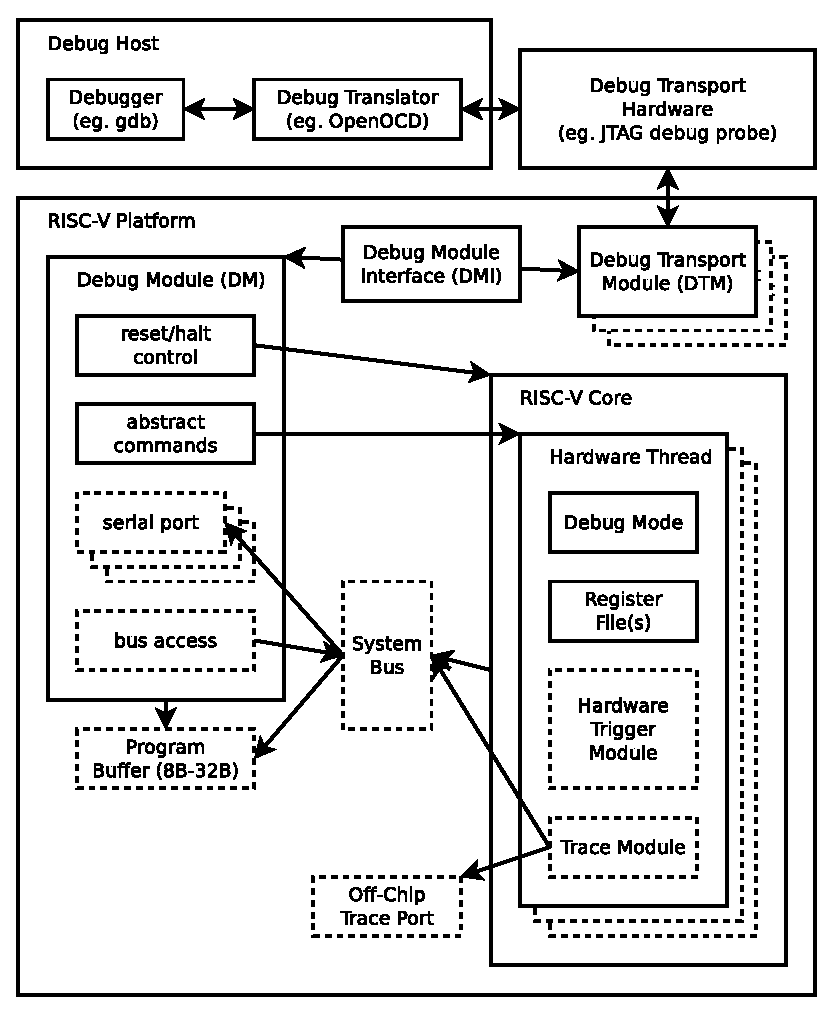
\includegraphics[width=\textwidth]{overview.eps}
   \caption{RISC-V Debug System Overview}
   \label{fig:overview}
\end{figure}

The user interacts with the Debug Host (eg. laptop), which is running a
debugger (eg. gdb).  The debugger communicates with a Debug Translator (eg.
OpenOCD, which may include a hardware driver) to communicate with Debug
Transport Hardware (eg.  Olimex USB-JTAG adapter) that's connected to the host.
The Debug Transport Hardware connects the Debug Host to the Platform's Debug
Transport Module (DTM).  The DTM provides access to the DM using the Debug
Module Interface (DMI).

The DM allows the debugger to halt any hart in the platform. Abstract commands
provide access to GPRs and possibly other registers. More complex harts will
require the Program Buffer be implemented, which the debugger uses to have the
hart execute arbitrary instructions while halted.

Each RISC-V core may implement a Trigger Module for each hart.  These can
implement breakpoints, which cause a hart to halt spontaneously.  When that
happens the DM notices because the hart will signal the DM that it's ready for
an instruction.

\section{Debug Transport Module (DTM)}

Debug Transport Modules provide access to the DM over one or more transports
(eg. JTAG or USB).

There may be multiple DTMs in a single platform. Ideally every component that
communicates with the outside world includes a DTM, allowing a platform to be
debugged through every transport it supports.  For instance a USB component
could include a DTM. This would trivially allow any platform to be debugged
over USB. All that is required is that the USB module already in use also has
access to the Debug Bus.

Using multiple DTMs at the same time is not supported. It is left to the user
to ensure this does not happen.

\section{Debug Module (DM)} \label{dm}

\begin{steps}{The Debug Module is the interface between specific debug
    operations and their implementation. It must support the following
    operations:}
\item Provide access to a reset signal that allows debugging out of reset.
\item Allow any individual hart to be halted.
\item Provide status on which harts are halted.
\item Feed a specific hart one instruction, and have that hart execute the
    instruction.
\item Give the debugger necessary information about the implementation. The user
    should not have to configure anything beyond how the debugger accesses the
    Debug Module.
\end{steps}

Optionally, an Instruction Buffer can repeatedly feed the same set of
instructions to a hart.

A single DM can debug up to 1024 harts.

\subsection{Debug Module Interface (DMI)}

The Debug Module Interface can be a trivial bus with one master and one slave,
or use a more full-featured bus like TileLink or the AMBA Advanced Peripheral
Bus. The details are left to the system designer.

The DMI uses between TODO and 32 address bits.  It supports read and write
operations, which may return an error. (Errors are only used by the optional
System Bus Access and Serial Port blocks.) TODO: The bottom of the address space is
used for the DM. Extra space can be used for custom debug devices, other cores,
additional DMs, etc.

TODO: The space is laid out so that small systems can get away with just 4
address bits. Using the Instruction Buffer requires 5 bits, and systems that
have many cores will want to implement 6 bits.

\begin{table}[htp]
    \centering
    \caption{Debug Module Interface Address Space}
    \label{tab:header}
    \begin{tabulary}{\textwidth}{|r|L|}
        \hline
        0x00 -- 0x3f & Registers described in Section~\ref{dmdebbus}. \\
        \hline
        0x40 -- 0x5f & If accessible, there are 1024 bits here, one for each
        hart that may exist in the system. If the hart is ready for the DM to
        feed it an instruction, the bit is 1. Otherwise the bit is 0. The bit
        for hart 0 is the LSB in the 32-bit word at 0x40. The bit for hart 1023
        is the MSB in the 32-bit word at 0x5f. \\
        \hline
    \end{tabulary}
\end{table}

\subsection{Reset Control} \label{reset}

This block is connected to a global reset signal, which can
reset, or hold in reset, every component in the platform,
except for the Debug Module and Debug
Transport Modules. The purpose of this feature is to allow debugging
programs from the first instruction executed, so exactly what is affected
by this reset is implementation dependent.

%MAW: Concrete example... FE310 has register which tells the core why
% it was reset. Examples are ``Power-on-Reset'',
% ``External Reset'', and
% ``Watchdog Reset''. Similarly, there is a ``wakeup cause'' register
% which tells the core why it woke up.
% I don't think you would want the debugger
% to affect the control flow of code based on reading these registers, so
% somehow this debugger-driven reset signal can't impact them.
% But I don't think that should be spelled out case-by-case in this spec,
% so I want to focus on the actual requirement more than saying exactly
% what this reset should do.
%
% Also, based on this, is it necessary to say something like Debug Module
% registers are ONLY reset based on Power-On-Reset or explicit
% Test-Logic-Reset, similar to JTAG
% specification? Otherwise how do you debug what happens on e.g.
% external reset (when someone hits reset button).
%

\subsection{Halt Control}

This block controls halt signals from the Debug Module to a hart.  It is used
to halt a hart, and let it run again.

For each hart the block contains a single bit that is accessible through to
\Fhalt in \Rdmcontrol. When a debugger wants to halt a hart, it writes 1 to
this bit, and then waits for \Fhalt in that register to go high.  To resume,
the debugger clears the bit, and waits for it to go low.

The Debug Module conceptually has a direct connection to the halt signal of
every hart that has one. When set or cleared, a hart must respond in less than
one second.  (How this is implemented is not further specified. A few clock
cycles will be a more typical latency.)

\subsection{Abstract Commands}

A debugger can execute abstract commands by writing the command to \Rcommand.
If a command takes an argument, the debugger must write it to the {\tt data}
registers before writing to \Rcommand. If a command returns a results, it is
placed in the {\tt data} registers when the command is complete. Which {\tt
data} registers are used is described in Table~\ref{tab:datareg}. Depending on
the implementation, it may be possible to perform abstract commands even when
the hart is not halted.

\begin{table}[htp]
    \centering
    \caption{Use of Data Registers}
    \label{tab:datareg}
    \begin{tabulary}{\textwidth}{|r|l|l|}
        \hline
        XLEN & arg0/return value (LSW to MSW) & arg1 (LSW to MSW) \\
        \hline
        32 & \Rdatazero & \Rdataone \\
        \hline
        64 & \Rdatazero, \Rdataone & \Rdatatwo, \Rdatathree \\
        \hline
        128 & \Rdatazero, \Rdataone, \Rdatatwo, \Rdatathree &
        \Rdatafour, \Rdatafive, \Rdatasix, \Rdataseven \\
        \hline
    \end{tabulary}
\end{table}

\begin{table}[htp]
    \centering
    \caption{Abstract Register Numbers}
    \label{tab:regno}
    \begin{tabulary}{\textwidth}{|r|l|}
        \hline
        0x0000 -- 0x0fff & CSRs \\
        \hline
        0x1000 -- 0x101f & GPRs \\
        \hline
        0x1020 -- 0x103f & Floating point registers \\
        \hline
    \end{tabulary}
\end{table}

\input{abstract_commands.tex}

\subsection{Program Buffer}

A debugger can write a small program to the optional Program Buffer, and then
execute it using some of the abstract commands. The programs must end with {\tt
ebreak} or {\tt ebreak.c}. While these programs are executed, the hart does not
leave Halt Mode (see Section~\ref{haltmode}).

Executing the Program Buffer may clobber \Rdpc. If that is the case, it must be
possible to read/write \Rdpc using an abstract command. The debugger must
attempt to save \Rdpc between halting and executing a Program Buffer, and then
resture \Rdpc before leaving Halt Mode.

\subsection{Serial Ports}

The Debug Module may implement up to 8 serial ports. They support basic flow
control and full duplex data transfer between a component and the debugger.
They can be used to communicate with a debug monitor running on a hart, for the
equivalent of printf debugging, to provide a simple CLI without requiring any
extra peripherals, or more generally to emulate devices that aren't present.
All these uses require software support, and are not further specified here.

\subsection{Sytem Bus Access}

In a minimal configuration a debugger can access the system bus by having a
RISC-V hart perform the accesses it requires. Optionally a Bus Access block may
be implemented. Because the System Bus Access block performs accesses directly
from the DM, it only uses physical addresses.

Implementing a System Bus Access block has several benefits.
First, it is possible to
access memory in a running system with minimal impact.  Second, it may improve
performance when downloading programs. (There is only a benefit if JTAG TCK is a
significant fraction of the RISC-V hart's clock speed.)  Third, it may provide
access to devices that a hart does not have access to. A hart may be unable to
access all devices in a system (eg. for security reasons) and in this case the
debugger needs another path to access them.

To keep implementing, configuring, and using a debugger as simple as possible,
systems should use the same memory map for each hart. That means that a given
address maps to the same device no matter which hart performs the access.
(Different harts may not all have permission to access the same devices.) If
different harts do have unique memory maps then the system should provide
access to all devices using the Sytem Bus Access block.
This will make implementing,
configuring, and using a debugger more complex so should be avoided if
possible.

\subsection{Security}

To protect intellectual property it may be desirable to lock access to the
Debug Module.  To allow access during a manufacturing process and not
afterwards, a reasonable solution could be to add a fuse bit to the Debug
Module that can be used to be permanently disable it. Since this is technology
specific, it is not further addressed in this spec.

Another option is to allow the DM to be unlocked only by users who  have an
access key. A simple mechanism is documented in Section~\ref{authdata0}. When
\Fauthenticated is clear, the DM must not interact with the rest of the
platform in any way.

\subsection{Debug Module DMI Registers} \label{dmdebbus}

\input{dm1_registers.tex}

\subsection{Debug Module Serial Registers} \label{dmsysbus}

TODO: Figure out where these registers should really live on the system bus,
and how to communicate that to software. Or maybe there are magic CSRs to
access them as well?

\input{dm2_registers.tex}

%\section{Device Tree Additions TODO}
%
%The device tree is a data structure in ROM that all RISC-V platforms should
%have. It contains a variety of information about every component in the
%platform. (As of June 18, 2016 it is not yet part of any RISC-V spec.)
%
%The device tree contains the hart IDs for each core. The debugger reads this
%information to determine how many harts there are in the platform, and what
%their IDs are. It should expose each hart to the user as a separately
%debuggable entity. (Usually it will be called either a thread or a core.)

\section{RISC-V Debug}

Modifications to the RISC-V core to support debug are kept to a minimum.  There
is a special execution mode (Halt Mode) and a few extra CSRs. The DM takes care
of the rest.

\subsection{Hart IDs}

External debug imposes a few limits on hart IDs. Every hart in the system must
have a unique ID. (There could be additional harts that reuse IDs, but only one
of the harts that share an ID can be debugged.) One of the harts must use ID 0.
The debugger needs this to access the config string to enumerate the remaining
harts in the system. Hart IDs should be less than 128 if the Debug Bus address
is 5 bits wide, or less than 1024 if that address is 6 or more bits wide.

\subsection{Halt Mode} \label{haltmode}

Halt Mode is a special processor mode used only when the core is halted for
external debugging. How Halt Mode is entered is implementation-specific.

\begin{steps}{While in Halt Mode:}
\item All operations happen in machine mode.
\item \Fmprv in \Rmstatus is ignored.
\item All interrupts are masked.
\item Exceptions don't update any registers.  That includes {\tt cause}, {\tt
    epc}, {\tt badaddr}, and \Rmstatus.  Instead exceptions just set \Fhmexc in
    \Rdcsr.
\item No trigger actions are taken.
\item Trace is disabled.
\item Cycle counters may be stopped, depending on \Fstopcycle in \Rdcsr.
\item Timers may be stopped, depending on \Fstoptime in \Rdcsr.
\item The {\tt wfi} instruction acts as a {\tt nop}.
\item Almost all instructions that change the privilege level have undefined
    behavior.  This includes {\tt ecall}, {\tt mret}, {\tt hret}, {\tt sret},
    and {\tt uret}.  (To change the privilege level, the debugger can write
    \Fprv in \Rdcsr.) The exception is {\tt ebreak}. When that is executed in
    Halt Mode, it halts the processor again but without updating \Rdpc.
\end{steps}

\subsection{Load-Reserved/Store-Conditional Instructions}

The reservation registered by an {\tt lr} instruction on a memory address may
be lost when entering Halt Mode or while in Halt Mode.  This means that there
may be no forward progress if Halt Mode is entered between {\tt lr} and {\tt
sc} pairs.

\subsection{Reset}

If the halt signal is asserted when a core comes out of reset, the core must
enter Debug Mode before executing any instructions, but after performing any
initialization that would usually happen before the first instruction is
executed.

\subsection{Core Debug Registers} \label{debreg}

The Core Debug Registers must be implemented for each hart being debugged.

\input{core_registers.tex}

\section{Trigger Module}

Triggers can cause a debug exception, entry into Halt Mode, or a trace action
without having to execute a special instruction. This makes them invaluable
when debugging code from ROM. They can trigger on execution of instructions at
a given memory address, or on the address/data in loads/stores.  These are all
features that can be useful without having the Debug Module present, so the
Trigger Module is broken out as a separate piece that can be implemented
separately.

\begin{steps}{Each trigger may support a variety of features. A debugger can
    build a list of all triggers and their features as follows:}
\item Write 0 to \Rtselect.
\item Read back \Rtselect to confirm this trigger exists. If not, exit.
\item Read \Rtdataone, and possible \Rtdatatwo and \Rtdatathree depending on the
    trigger type.
\item If \Ftype in \Rtdataone was 0, then there are no more triggers.
\item Repeat, incrementing the value in \Rtselect.
\end{steps}

\subsection{Trigger Registers}

\input{hwbp_registers.tex}

\section{JTAG Debug Transport Module}

This Debug Transport Module is based around a normal JTAG Test Access Port
(TAP).  The JTAG TAP allows access to arbitrary JTAG registers by first
selecting one using the JTAG instruction register (IR), and then accessing it
through the JTAG data register (DR).

\subsection{Background}

JTAG refers to IEEE Std 1149.1-2013. It is a standard that defines test logic
that can be included in an integrated circuit to test the interconnections
between integrated circuits, test the integrated circuit itself, and observe or
modify circuit activity during the component’s normal operation. We're using it
for the third case here.  The standard defines a Test Access Port (TAP) that
can be used to read and write a few custom registers, which can be used to
communicate with debug hardware in a component.

\subsection{JTAG Connector}

Every target's JTAG connector seems to have its own pinout. To make it easy to
acquire debug hardware, this spec recommends a connector that is compatible
with the Cortex Debug Connector, as described below.

The connector is a .05"-spaced, gold-plated male header with .016" thick
hardened copper or beryllium bronze square posts (SAMTEC FTSH-105 or
equivalent). Female connectors are compatible \SI{20}{\micro\metre} gold
connectors in order to prevent oxide build-up on tin connectors.

Viewing the male header from above (the pins pointing at your eye), a target's
connector looks as it does in Table~\ref{tab:header}. The function of each pin
is described in Table~\ref{tab:pinout}.

%MAW: Why do we only have 'RESET', but no 'TRST(n)' signal?
% See http://openocd.org/doc/html/Reset-Configuration.html
% Both are useful.
% One is explicitly ``test logic reset'', which would imply
% resetting the JTAG state machine and all associated test logic, in this
% case the Debug Transport Module, synchronizers, and perhaps even
% the Debug Module itself. It basically does the same thing as getting
% the JTAG state machine into TEST_LOGIC_RESET state, which is
% why it is optional.
%
% The other is a convenience which allows the debugger to essentially
% hit the system reset button, which is basically mutually exclusive from
% what TRST resets.
%
% I think a common workflow would be
% to assert the halt signal in Debug Module,
% then tell the debugger to pull the 'RESET' signal.
% The desired effect woudld be to be able to debug the
% code that executes on external reset.
%
% Another common workflow would be to have been debugging for a while,
% then you disconnect the debugger.
% Another user connects, and has no idea what state the debug logic
% is in. They could assert the TRSTn signal (or clock JTAG TAP into
% the proper state) and then know that all the Debug Transport Module
% (and Debug Module logic...?) is in a known state.
%

\begin{table}[htp]
    \centering
    \caption{JTAG Connector Diagram}
    \label{tab:header}
    \begin{tabulary}{\textwidth}{|r|r|r|l|}
        \hline
        VCC & 1 & 2 & TMS \\
        \hline
        GND & 3 & 4 & TCK \\
        \hline
        GND & 5 & 6 & TDO \\
        \hline
        KEY & 7 & 8 & TDI \\
        \hline
        N/C & 9 & 10 & RESET \\
        \hline
    \end{tabulary}
\end{table}

\begin{table}[htp]
    \centering
    \caption{JTAG Connector Pinout}
    \label{tab:pinout}
    \begin{tabulary}{\textwidth}{|r|l|L|}
        \hline
        1 & VCC & Power provided by the target, which may be used to power the
        debug adapter. Must be able to source at least 25mA. This signal also
        serves as the reference voltage for logic high.

        This pin must be clearly marked in both male and female headers.\\
        \hline
        2 & TMS & JTAG TMS signal, driven by debug adapter. \\
        \hline
        3 & GND & Target ground. \\
        \hline
        4 & TCK & JTAG TCK signal, driven by the debug adapter. \\
        \hline
        5 & GND & Target ground. \\
        \hline
        6 & TDO & JTAG TDO signal, driven by the target. \\
        \hline
        7 & KEY & This pin should be clipped in male connectors, and plugged in
        female connectors. Electrically it must not be connected. \\
        \hline
        8 & TDI & JTAG TDI signal, driven by the debug adapter.

        This pin may be used by a target to sense a debugger at reset by weakly
        pulling this signal high during a brief detection period at reset.
        Debuggers should drive TDI low when the interface is idle. \\
        \hline
        9 & N/C & Not connected in either target or debug adapter. May be used
        in future specs. \\
        \hline
        10 & RESET & Reset signal, driven by the debug adapter. This may be
        active low or active high, depending on the target's requirements. A
        debug adapter must accommodate either option. Asserting reset should
        reset any RISC-V cores as well as any other peripherals on the PCB.
        It should not reset the debug logic.
        If not implemented in a target, this pin must not be connected. \\
        \hline
    \end{tabulary}
\end{table}

Target connectors may be shrouded. In that case the key slot should be next to
pin 5. Female headers should have a matching key.

Debug adapters should be tagged or marked with their isolation voltage
threshold (i.e. unisolated, 250V, etc.).

All debug adapter pins other than GND should be current-limited to 20mA.

\subsection{JTAG Registers}

JTAG DTMs should use a 5-bit JTAG IR. When the TAP is reset, IR must default to
00001, selecting the IDCODE instruction. A full list of JTAG registers along
with their encoding is in Table~\ref{table:jtag_registers}. The only regular
JTAG registers a debugger might use are BYPASS and IDCODE, but the JTAG
standard recommends a lot of other instructions so we leave IR space for them.
If they are not implemented, then they must select the BYPASS register.

\input{jtag_registers.tex}

\newpage
\appendix

\section{Hardware Implementations}

Below are three possible implementations. A designer could choose one, mix and
match, or come up with their own design.

\subsection{Direct}

Halting happens by inhibiting instruction fetching in Halt Mode.

Muxes on the register file(s) allow for implementing those abstract commands.
(TODO: Should we spec a suggested way of communicating between DM and hart, so
that a reusable DM can be implemented?)

To execute a program buffer, force \Rpc to the start of it, and re-enable
instruction fetching (while staying in Halt Mode) until {\tt ebreak} is
encountered.

\Rdpc is not physically a CSR. Instead, accessing it directly access \Rpc.

\subsection{Plain Exception}

In this implementation, Halt Mode acts more like a real exception, jumping to a
memory region that is serviced by the DM. When taking this exception, \Rpc is
saved to \Rdpc. To allow the DM to individually control one out of several
halted harts, each hart jumps to a hard-coded unique address.

\Rdatazero etc. are mapped into regular memory at address 0x400. The important
property of that address is that it's reachable relative to \Rzero. The exact
address is an implementation detail that a debugger must not rely on.

When first halting, the loop looks like this:
\begin{minted}{gas}
dm_control_hart_0:
        nop
        j       dm_park_hart_0
\end{minted}

The DM assumes that every instruction fetched from it is executed.

To implement the abstract GPR access instructions, the {\tt nop} is changed
(for a single fetch) to {\tt lw <gpr>, 0x400(zero)} or {\tt sw 0x400(zero),
<gpr>}. To execute the Program Buffer, the {\tt nop} is changed to {\tt j
dm\_program\_buffer}. To resume execution, the {\tt nop} is changed to {\tt
dret}.

When {\tt dret} is executed, \Rpc is restored from \Rdpc and normal execution
resumes at the privilege set by \Fprv.

\section{Debugger Implementation}

This section details how an external debugger might use the described debug
interface to perform some common operations on RISC-V cores using the JTAG DTM.
All these examples assume a 32-bit core but it should be easy to adapt the
examples to 64- or 128-bit cores.

To keep the examples readable, they all assume that everything succeeds, and
that they complete faster than the debugger can perform the next access. This
will be the case in a typical JTAG setup. However, the debugger must always
check the sticky error status bits after performing a sequence of actions. If
it sees any that are set, then it should attempt the same actions again,
possibly while adding in some delay, or explicit checks for status bits.

\subsection{Debug Bus Access} \label{dbusaccess}

To read an arbitrary Debug Bus register, select \Rdbus, and scan in a value
with \Fop set to 1, and \Faddress set to the desired register address. In
Update-DR the operation will start, and in Capture-DR its results will be
captured into \Fdata.  If the operation didn't complete in time, \Fop will be 3
and the value in \Fdata must be ignored. The error condition must be cleared by
writing \Fdbusreset in \Rdtmcontrol, and then the operation must be tried
again. This time the debugger should allow for more time between Capture-DR and
Update-DR.

To write an arbitrary Debug Bus register, select \Rdbus, and scan in a value
with \Fop set to 2, and \Faddress and \Fdata set to the desired register
address and data respectively. From then on everything happens exactly as with
a read, except that a write is also performed right after the read. The
operation isn't considered complete until the write has happened.

It should almost never be necessary to scan IR, avoiding a big part of the
inefficiency in typical JTAG use.

\subsection{Main Loop}

A debugger continuously monitors \Rhaltsum to see if any harts have spontaneously
halted.

\subsection{Halting}

To halt a hart, the debugger sets \Fhartid and \Fhalt. Then it waits for \Fhalt
to become set.

\subsection{Accessing Registers}

\subsubsection{Using Abstract Command}

\begin{table}[htp]
    \centering
    \caption{Read \Szero using abstract command}
    \begin{tabulary}{\textwidth}{|r|r|r|L|}
        \hline
        Op & Address & Value & Comment \\
        \hline
        Write & \Rcommand & 0x1008 & Read \Szero \\
        \hline
        Read & \Rdatazero & - & Returns value that was in \Szero \\
        \hline
    \end{tabulary}
\end{table}

\begin{table}[htp]
    \centering
    \caption{Write \Rmstatus using abstract command}
    \begin{tabulary}{\textwidth}{|r|r|r|L|}
        \hline
        Op & Address & Value & Comment \\
        \hline
        Write & \Rdatazero & new value & \\
        \hline
        Write & \Rcommand & 0x10300 & Write \Rmstatus \\
        \hline
    \end{tabulary}
\end{table}

\subsubsection{Using Program Buffer}

Abstract commands are used to exchange data with GPRs. Using this mechanism, other
registers can be accessed by moving their value into/out of GPRs.

\begin{table}[htp]
    \centering
    \caption{Write \Rmstatus using program buffer}
    \begin{tabulary}{\textwidth}{|r|r|r|L|}
        \hline
        Op & Address & Value & Comment \\
        \hline
        Write & \Ribufzero & {\tt csrw s0, MSTATUS} & \\
        \hline
        Write & \Ribufone & {\tt ebreak} & \\
        \hline
        Write & \Rdatazero & new value & \\
        \hline
        Write & \Rcommand & 0x31008 & Write \Szero, then execute program buffer \\
        \hline
    \end{tabulary}
\end{table}

\begin{table}[htp]
    \centering
    \caption{Read \Fone using program buffer}
    \begin{tabulary}{\textwidth}{|r|r|r|L|}
        \hline
        Op & Address & Value & Comment \\
        \hline
        Write & \Ribufzero & {\tt fmv.x.s s0, f1} & \\
        \hline
        Write & \Ribufone & {\tt ebreak} & \\
        \hline
        Write & \Rcommand & 0x41008 & Execute program buffer, then read \Szero \\
        \hline
        Read & \Rdatazero & - & Returns the value that was in \Fone \\
        \hline
    \end{tabulary}
\end{table}

\subsection{Reading Memory}

\subsubsection{Using System Bus Access}

\subsubsection{Using Program Buffer}

\begin{table}[htp]
    \centering
    \caption{Read from memory using program buffer}
    \begin{tabulary}{\textwidth}{|r|r|r|L|}
        \hline
        Op & Address & Value & Comment \\
        \hline
        Write & \Ribufzero & {\tt lw s0, 0(s0)} & \\
        \hline
        Write & \Ribufone & {\tt ebreak} & \\
        \hline
        Write & \Rdatazero & address & \\
        \hline
        Write & \Rcommand & 0x31008 & Write \Szero, then execute program buffer \\
        \hline
        Write & \Rcommand & 0x1008 & Read \Szero \\
        \hline
        Read & \Rdatazero & - & Value read from memory \\
        \hline
    \end{tabulary}
\end{table}

\begin{table}[htp]
    \centering
    \caption{Read block of memory using program buffer}
    \begin{tabulary}{\textwidth}{|r|r|r|L|}
        \hline
        Op & Address & Value & Comment \\
        \hline
        Write & \Ribufzero & {\tt lw s1, 0(s0)} & \\
        \hline
        Write & \Ribufone & {\tt addi s0, s0, 4} & \\
        \hline
        Write & \Ribuftwo & {\tt ebreak} & \\
        \hline
        Write & \Rdatazero & address & \\
        \hline
        Write & \Rcommand & 0x31008 & Write \Szero, then execute program buffer \\
        \hline
        Write & \Rcommand & \Fexeca OR 0x1009 & Read \Sone, then execute program buffer \\
        \hline
        Write & \Rabstractcs & \Fautoexeczero OR \Fcmderr & Set \Fautoexeczero \\
        \hline
        Read & \Rdatazero & - & Get value read from memory, then execute program buffer \\
        \hline
        Read & \Rdatazero & - & Get next value read from memory, then execute program buffer \\
        \hline
        ... & ... & ... & ... \\
        \hline
        Write & \Rabstractcs & \Fcmderr & Clear \Fautoexeczero \\
        \hline
        Read & \Rdatazero & - & Get last value read from memory. \\
        \hline
    \end{tabulary}
\end{table}

TODO: Table~\ref{tab:memread} shows the scans involved in reading a single word using
this method.

\begin{table}[htp]
    \centering
    \caption{Memory Read Timeline}
    \label{tab:memread}
    \begin{tabulary}{\textwidth}{|r|l|L|}
        \hline
        & JTAG State & Activity \\
        \hline
        TODO & TODO & TODO \\
%        1 & Shift-DR & Debugger shifts in write of 0x41002403 to dram[0], and
%        gets back the result of whatever happened previously. \\
%        & Update-DR & DTM starts read from dram[0], followed by write to
%        dram[0]. \\
%        \hline
%        2 & Capture-DR & DTM captures results of read from dram[0]. \\
%        & Shift-DR & Debugger shifts in write of 0x42483 to dram[1], and gets
%        back the old contents of the first word in Debug RAM. \\
%        & Update-DR & DTM starts read from dram[1], followed by write to
%        dram[1]. \\
%        \hline
%        3 & Capture-DR & DTM captures results of read from dram[1]. \\
%        & Shift-DR & Debugger shifts in write of 0x40902823 to dram[2], and
%        gets back the old contents of the second word in Debug RAM. \\
%        & Update-DR & DTM starts read from dram[2], followed by write to
%        dram[2]. \\
%        \hline
%        4 & Capture-DR & DTM captures results of read from dram[2]. \\
%        & Shift-DR & Debugger shifts in write of 0x3f80006f to dram[3], and
%        gets back the old contents of the third word in Debug RAM. \\
%        & Update-DR & DTM starts read from dram[3], followed by write to
%        dram[3]. \\
%        \hline
%        5 & Capture-DR & DTM captures results of read from dram[3]. \\
%        & Shift-DR & Debugger shifts in write of the address the user wants to
%        read from to dram[4], using the interrupting Debug RAM register to assert
%        the Debug Interrupt. The old contents of the fourth word in Debug RAM
%        are shifted out. \\
%        & Update-DR & DTM starts read from dram[4], followed by write to
%        dram[4], and then sets the interrupt bit. The hart will respond to the
%        Debug Interrupt by executing the program in Debug RAM which in this
%        case will read the address written, and replace the entry in Debug RAM
%        with the data at that address. \\
%        \hline
%        6 & Capture-DR & DTM captures results of read from dram[4]. \\
%        & Shift-DR & Debugger shifts in read from dram[4], and gets back the
%        old contents of the fourth word in Debug RAM. (This is the value that
%        was there just before the address was written there.) \\
%        & Update-DR & DTM starts read from dram[4]. \\
%        \hline
%        7 & Capture-DR & DTM captures results of read from dram[4]. \\
%        & Shift-DR & Debugger shifts in nop, and gets back the contents of the
%        fourth word in Debug RAM. This is the value that was there during the
%        previous Update-DR, which is the result of the Debug Program execution.
%        \\
        \hline
    \end{tabulary}
\end{table}

\subsection{Writing Memory} \label{writemem}

TODO: Just like reading memory.

\begin{commentary}
    % Select-DR-Scan to Shift-DR: 2
    % Shift-DR to Exit1-DR: dbus register is abits+33 bits, so 38
    % Exit1-DR to Select-DR-Scan: 2
    % Total: 42

    TODO: maybe update

    After the instruction buffer is configured, each word can be written to the
    target in 42 TCK cycles. That's 76\% efficient, and translates to a
    download speed of 930KB/s at a 10MHz TCK.  That should be good enough that
    it's not worth making the JTAG interface more complex to improve the
    efficiency. (This assumes the Debug Bus uses 5 address bits and that the
    debugger never has to wait for the core.)
\end{commentary}

\subsection{Running}

First, the debugger should restore any registers that it has clobbered.  Once
that's done, it can let the core run by clearing \Fhalt.

\subsection{Single Step}

A debugger can single step the core by setting a breakpoint on the next
instruction and letting the core run, or by asking the hardware to perform a
single step. The former requires the debugger to have much more knowledge of
the hardware than the latter, so the latter is preferred.

Using the hardware single step feature is almost the same as regular running.
The debugger just sets \Fstep in \Rdcsr before letting the core run. The core
behaves exactly as in the running case, except that interrupts are left off and
it only fetches and executes a single instruction before re-entering Debug
Mode.

\subsection{Handling Exceptions}

Generally the debugger can avoid exceptions by being careful with the programs
it writes. Sometimes they are unavoidable though, eg. if the user asks to
access memory or a CSR that is not implemented. A typical debugger will not
know enough about the platform to know what's going to happen, and must attempt
the access to determine the outcome.

When an exception occurs in Halt Mode, \Fhmexc becomes set. If the debugger did
something that might have caused an exception, it should check for that. If
there was an exception, it's left to the debugger to know what must have caused
it.

\subsection{Quick Access} \label{quickaccess}

TODO

\section{Trace Module}

{\bf This part of the spec needs work before it's ready to be implemented,
which is why it's in the appendix. It's left here to give a rough idea of some
of the issues to consider.}

Aside from viewing the current state of a core, knowing what happened in the
past can be incredibly helpful. Capturing an execution trace can give a user
that view.  Unfortunately processors run so fast that they generate trace data
at a very large rate. To help deal with this, the trace data format allows for
some simple compression.

The trace functionality described here aims to support 3 different use cases:
\begin{enumerate}
    \item Full reconstruction of all processor state, including register values
        etc. To achieve this goal the decoder will have to know what code is
        being executed, and know the exact behavior of every RISC-V
        instruction.
    \item Reconstruct just the instruction stream. Get enough data from the
        trace stream that it is possible to make a list of every instruction
        executed.  This is possible without knowing anything about the code or
        the core executing it.
    \item Watch memory accesses for a certain memory region.
\end{enumerate}

Trace data may be stored to a special on-core RAM, RAM on the system bus, or to
a dedicated off-chip interface. Only the system RAM destination is covered
here.

\subsection{Trace Data Format}

Trace data should be both compact and easy to generate. Ideally it's also easy
to decode, but since decoding doesn't have to happen in real time and will
usually have a powerful workstation to do the work, this is the least important
concern.

Trace data consists of a stream of 4-bit packets, which are stored in memory in
32-bit words by putting the first packet in bits 3:0 of the 32-bit word, the
second packet into bits 7:4, and so on. Trace packets and their encoding are
listed in Table~\ref{tab:tracepackets}.

\begin{table}[htp]
   \centering
   \caption{Trace Sequence Header Packets}
   \label{tab:tracepackets}
   \begin{tabulary}{\textwidth}{|l|l|L|}
      \hline
      0000 & Nop & Packet that indicates no data. The trace source must use
      these to ensure that there are 8 synchronization points in each buffer. \\
      \hline
      0001 & PC & Followed by a Value Sequence containing bits XLEN-1:1 of the
      PC if the compressed ISA is supported, or bits XLEN-1:2 of the PC if the
      compressed ISA is not supported.
      Missing bits must be filled in with the last PC value. \\
      \hline
      0010 & Branch Taken & \\
      \hline
      0011 & Branch Not Taken & \\
      \hline
      0100 & Trace Enabled & Followed by a single packet indicating the version
      of the trace data (currently 0). \\
      \hline
      0101 & Trace Disabled & Indicates that trace was purposefully disabled,
      or that some sequences were dropped because the trace buffer overflowed. \\
      \hline
      0110 & Privilege Level & Followed by a packet containing whether the
      cause of the change was an interrupt (1) or something else (0) in bit 3,
      PRV[1:0] in bits 2:1, and IE in bit 0. \\
      \hline
      0111 & Change Hart & Followed by a Value Sequence containing the hart ID
      of the hart whose trace data follows. Missing bits must be filled in with
      0. \\
      \hline
      1000 & Load Address & Followed by a Value Sequence containing the
      address.  Missing bits must be filled in with the last Load Address
      value. \\
      \hline
      1001 & Store Address & Followed by a Value Sequence containing the
      address. Missing bits must be filled in with the last Store Address
      value. \\
      \hline
      1010 & Load Data & Followed by a Value Sequence containing the data.
      Missing bits must be filled in by sign extending the value. \\
      \hline
      1011 & Store Data & Followed by a Value Sequence containing the data.
      Missing bits must be filled in by sign extending the value. \\
      \hline
      1100 & Timestamp & Followed by a Value Sequence containing the timestamp.
      Missing bits should be filled in with the last Timestamp value. \\
      \hline
      1101 & Reserved & Reserved for future standards. \\
      \hline
      1110 & Custom & Reserved for custom trace data. \\
      \hline
      1111 & Custom & Reserved for custom trace data. \\
      \hline
   \end{tabulary}
\end{table}

Several header packets are followed by a Value Sequence, which can encode
values between 4 and 64 bits. The sequence consists first of a 4-bit size
packet which contains a single number N.  It is followed by N+1 4-bit packets
which contain the value. The first packet contains bits 3:0 of the value. The
next packet contains bits 7:4, and so on.

\subsection{Trace Events}

Trace events are events that occur when a core is running that result in trace
packets being emitted. They are listed in Table~\ref{tab:traceevents}.

\begin{table}[htp]
   \centering
   \caption{Trace Data Events}
   \label{tab:traceevents}
   \begin{tabulary}{\textwidth}{|l|L|}
      \hline
      Opcode & Action \\
      \hline
      {\tt jal} & If \Femitbranch is disabled but \Femitpc is enabled, emit
      2 PC values: first the address of the instruction, then the address being
      jumped to. \\
      \hline
      {\tt jalr} & If \Femitbranch is disabled but \Femitpc is enabled, emit 2 PC
      values: first the address of the instruction, then the address being
      jumped to. Otherwise, if \Femitstoredata is enabled emit just the
      destination PC. \\
      \hline
      BRANCH & If \Femitbranch is enabled, emit either Branch Taken or Branch
      Not Taken.  Otherwise if \Femitpc is enabled and the branch is taken,
      emit 2 PC values: first the address of the branch, then the address being
      branched to. \\
      \hline
      LOAD & If \Femitloadaddr is enabled, emit the address.  If
      \Femitloaddata is enabled, emit the data that was loaded. \\
      \hline
      STORE & If \Femitstoreaddr is enabled, emit the address. If
      \Femitstoredata is enabled, emit the data that is stored. \\
      \hline
      Traps & {\tt scall}, {\tt sbreak}, {\tt ecall}, {\tt ebreak}, and {\tt
      eret} emit the same as if they were {\tt jal} instructions. In addition they
      also emit a Privilege Level sequence. \\
      \hline
      Interrupts & Emit PC (if enabled) of the last instruction executed.  Emit
      Privilege Level (if enabled).  Finally emit the new PC (if enabled). \\
      \hline
      CSR instructions & For reads emit Load Data (if enabled). For writes emit
      Store Data (if enabled). \\
      \hline
      Data Dropped & After packet sequences are dropped because data is
      generated too quickly, Trace Disabled must be emitted. It's not necessary
      to follow that up with a Trace Enabled sequence. \\
      \hline
   \end{tabulary}
\end{table}

\subsection{Synchronization}

If a trace buffer wraps, it is no longer clear what in the buffer is a header
and what isn't. To guarantee that a trace decoder can sync up easily, each
trace buffer must have 8 synchronization points, spaced evenly throughout the
buffer, with the first one at the very start of the buffer. A synchronization
point is simply an address where there is guaranteed to be a sequence header.
To make this happen, the trace source can insert a number of Nop headers into
the sequence just before writing to the synchronization point.

Aside from synchronizing a place in the data stream, it's also necessary to
send a full PC, Read Address, Write Address, and Timestamp in order for those
to be fully decoded. Ideally that happens the first time after every
synchronization point, but bandwidth might prevent that. A trace source should
attempt to send one full value for each of these (assuming they're enabled)
soon after each synchronization point.

\subsection{Trace Registers}

\input{trace_registers.tex}

\section{Future Ideas}
Some future version of this spec may implement some of the following features.

\begin{enumerate}
   \item The spec defines several additions to the Device Tree which enable a
      debugger to discover hart IDs and supported triggers for all the cores
      in the system.
   \item DTMs can function as general bus slaves, so they would look like
      regular RAM to bus masters.
   \item Harts can be divided into groups. All the harts in the same group can
      be halted/run/stepped simultaneously. When a hart hits a breakpoint, all
      the other harts in the same group also halt within a few clock cycles.
   \item DTMs are specified for protocols like USB, I2C, SPI, and SWD.
   \item Core registers can be read without halting the processor.
   \item The debugger can communicate with the power manager to power cores up
      or down, and to query their status.
   \item Serial ports can raise an interrupt when a send/receive queue becomes full/empty.
   \item The debug interrupt can be masked by running code. If the interrupt is
      asserted, then deasserted, and then asserted again the debug interrupt
      happens anyway. This mechanism can be used to eg. read/write memory with
      minimal interruption, making sure never to interrupt during a critical
      piece of code.
   \item The debugger can non-intrusively sample a recent PC value from any
      running hart.
\end{enumerate}

\section{Change Log}

\begin{versionhistory}
    \input{changelog.tex}
\end{versionhistory}

\end{document}
